\documentclass[10pt]{article}

%\mode<presentation>{}
\usepackage[utf8]{inputenc}
\usepackage{graphicx}
\usepackage{tikz}
\usepackage{tcolorbox}
\usepackage[absolute,overlay]{textpos}
\usepackage{changepage}
\usepackage{xcolor}
%\tikzstyle{every node} = [align=center]
\usepackage{helvet}
%\usepackage{sansmathfonts}
\usepackage{amsmath}
\renewcommand{\familydefault}{\sfdefault}

\newcommand\BWone{4}
\newcommand\BWtwo{3.5}
\newcommand\BWthree{2.1}
\newcommand\BHone{0.2}
\newcommand\BHtwo{1}
\newcommand\BHthree{1.1}
\newcommand\Hone{-4}
\newcommand\Htwo{4}
\newcommand\Hthree{5.5}

\newcommand\Vone{1}

\newcommand\Vtwo{-6}

\newcommand\Vthree{-8.3}

\newcommand\HGap{0.1}
\newcommand\Vgap{1}

\newcommand\Loffset{0.3}

\definecolor{boxcolor}{HTML}{fab71b}
\definecolor{title1}{HTML}{0070c0}
\definecolor{title2}{HTML}{2f5496}

\begin{document}

%\begin{frame}

\begin{adjustwidth}{-6em}{}

\begin{tikzpicture}
  \node[anchor=north ] at (\Hone-\BWone -\Loffset,\Vone+\BHone+1+\Loffset) {\Large a}; 
  \node[anchor=north] at (\Hone,\Vone-0.4) {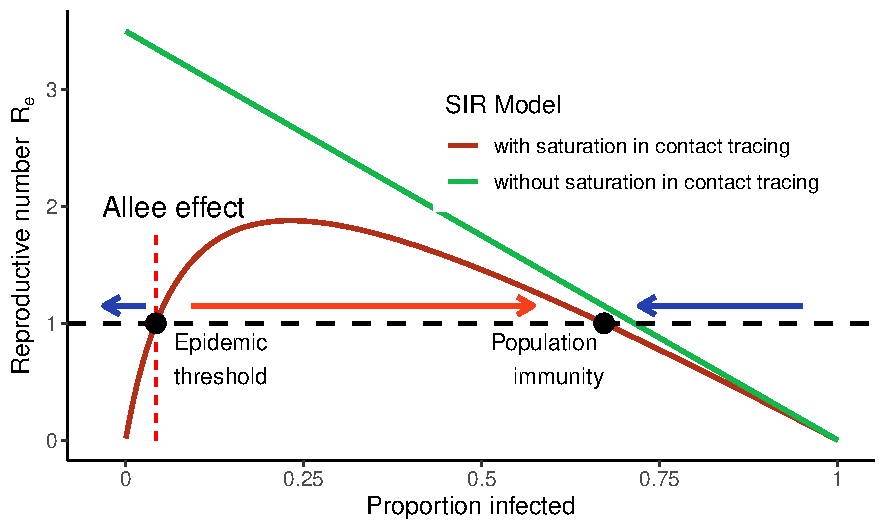
\includegraphics[width=0.6\textwidth]{../allee1D.pdf}};
   \draw[fill = boxcolor, draw=none]  (\Hone-\BWone,\Vone-\BHone ) rectangle (\Hone+\BWone,\Vone+\BHone)
   

       node[pos=0.5] {\scriptsize $R_e = P_{susceptible} \cdot b_{link} (L \cdot f_{q} + L_{max} \cdot f_{nq})$};

       \fill[title1] (\Hone-\BWone,\Vone+1) rectangle (\Hone+\BWone,\Vone+\BHone)
       node[pos=0.5,align=center,font=\scriptsize, color=white] {Non-pharmaceutical interventions (NPIs) \\ induce an Allee effect on disease dynamics};
;
\node[anchor=north ] at (\Htwo-\BWone -\Loffset+\Vgap,\Vone+\BHone+1+\Loffset) {\Large b}; 

       
  \fill[title2]  (\Htwo-\BWone+\Vgap,\Vone-\BHone) rectangle (\Htwo+\BWone+\Vgap,\Vone+1)
    node[pos=0.5,align=center,font=\scriptsize, color=white] {Transition between dynamic states is determined by the \\ strength of NPIs and the proportion of infected individuals};

  \node[anchor=north] at (\Htwo,\Vone-0.2) {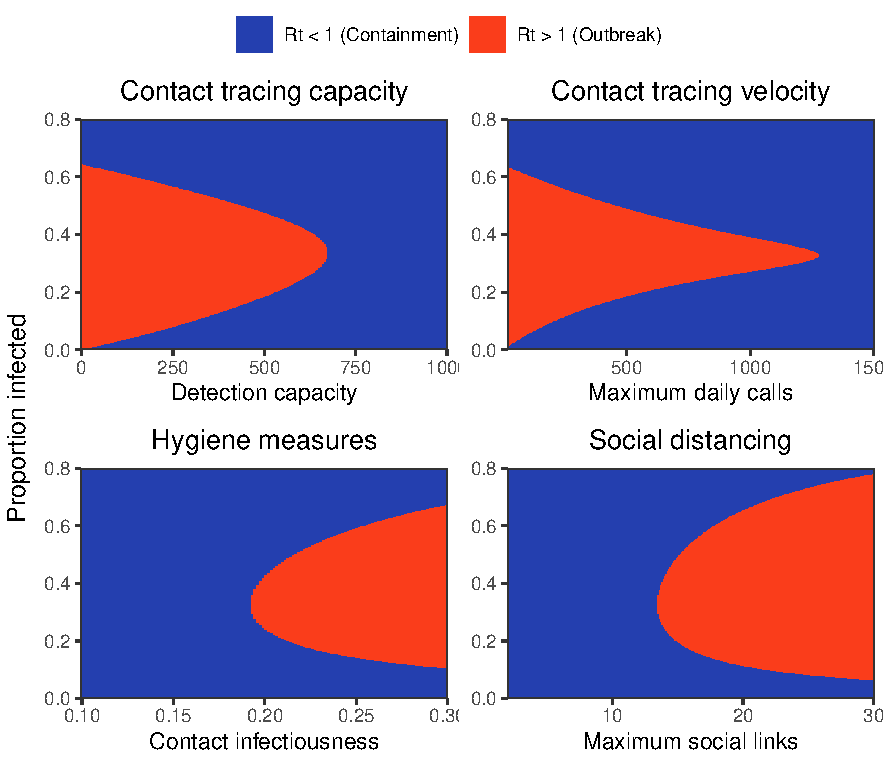
\includegraphics[width=0.55\textwidth]{../phase_space.pdf}};

 \node[anchor=north ] at (\Hone-\BWone -\Loffset,\Vtwo+\BHtwo+1+\Loffset) {\Large c}; 

   \fill[title2]  (\Hone-\BWone,\Vtwo-\BHone+1) rectangle (\Hone+\BWone,\Vtwo+1.8)
    node[pos=0.5,align=center,font=\scriptsize, color=white] {Simulated dynamics with an NPI-induced Allee effect \\ often show sharp accelerationsafter slow initial spread};

  
  \draw[fill=boxcolor,draw=none]  (\Hone-\BWone,\Vtwo-\BHtwo) rectangle (\Hone+\BWone,\Vtwo+\BHtwo)
    node[pos=0.5,align=left,font=\tiny] {\bf Simulated SIR Dynamics \\
    $S(t+1) = S(t) - I_{new}(d)$ \\
    $I(t+1) = I(t) + I_{new}(t) - \frac{I(t)}{\gamma(I(t))} + I_{imp}(t) $ \\
    $R(t+1) = R(t) + \frac{I(t)}{\gamma(I(t))} $ \\
    $I_{new}(t)\sim {\rm Poisson}(\lambda) $, $\lambda= \frac{\beta(I(t)) I(t)^p S(t)}{N} $ \\
    $I_{imp}(t) \sim NB (\mu, \sigma) $};

  \node[anchor=north] at (\Hone+0.5,\Vtwo-1) {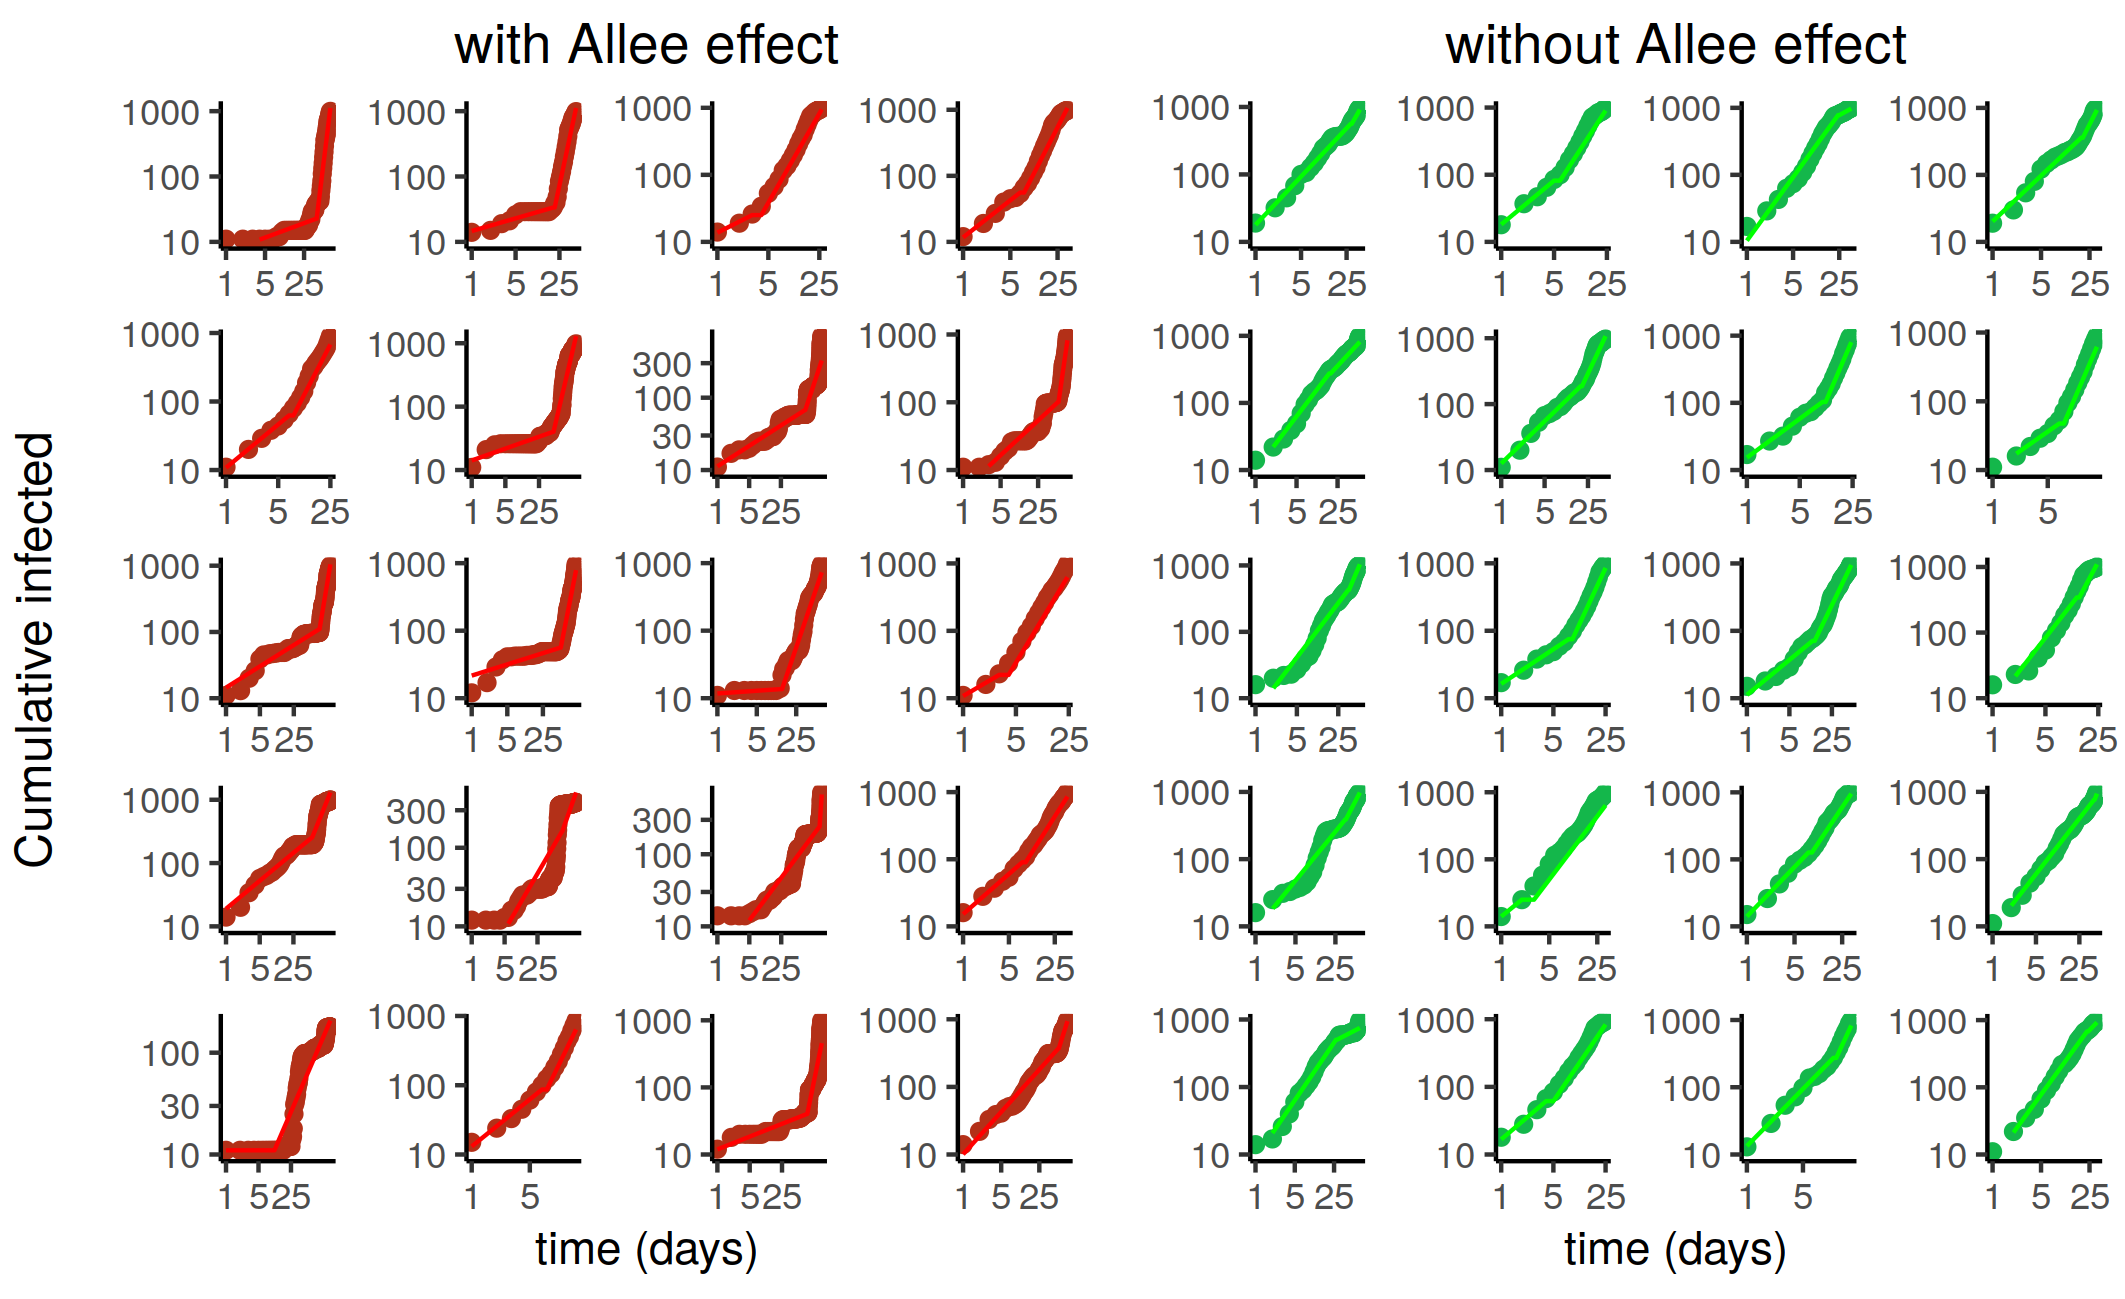
\includegraphics[width=0.68\textwidth]{../simDynamics.png}};

  \node[anchor=north ] at (\Htwo-\BWone -\Loffset+\Vgap,\Vtwo+\BHtwo -.8 ) {\Large d}; 

  \node[anchor=north] at (\Htwo+0.5,\Vtwo+1) {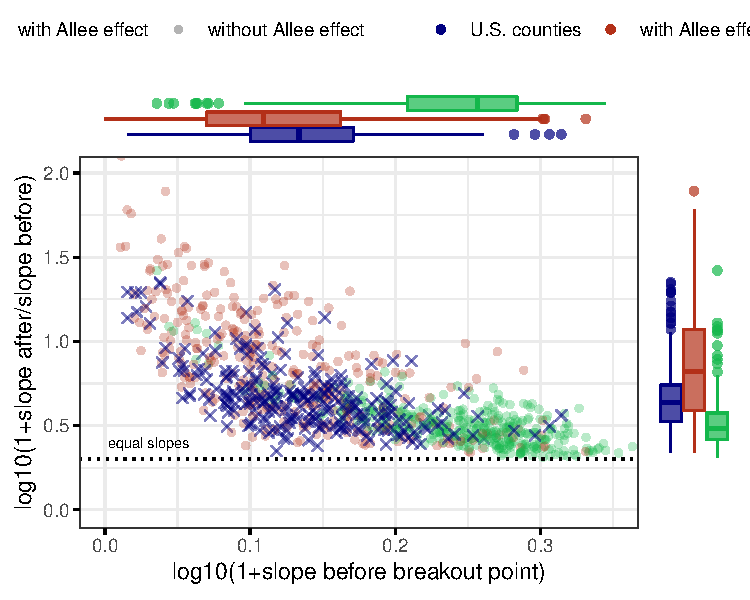
\includegraphics[width=0.6\textwidth]{../scatter_condados.pdf}};


\end{tikzpicture}

\end{adjustwidth}


\end{document}





